
%***************************************************************************
%
% CreditCruncher - A portfolio credit risk valorator
% Copyright (C) 2004 Gerard Torrent
%
% This program is free software; you can redistribute it and/or
% modify it under the terms of the GNU General Public License
% as published by the Free Software Foundation; either version 2
% of the License.
%
% This program is distributed in the hope that it will be useful,
% but WITHOUT ANY WARRANTY; without even the implied warranty of
% MERCHANTABILITY or FITNESS FOR A PARTICULAR PURPOSE.  See the
% GNU General Public License for more details.
%
% You should have received a copy of the GNU General Public License
% along with this program; if not, write to the Free Software
% Foundation, Inc., 59 Temple Place - Suite 330, Boston, MA 02111-1307, USA.
%
%
% resolution.tex - TeX documentation file
% --------------------------------------------------------------------------
%
% 2005/01/22 - Gerard Torrent [gerard@fobos.generacio.com]
%   . initial release
%
%***************************************************************************

\chapter{Resoluci\'on del problema}
\label{sec:resolution}

En este cap\'itulo se establecen las hip\'otesis de trabajo, se introducen los
elementos usados para la resoluci\'on y se describen dos m\'etodos de
resoluci\'on basados en simulaci\'on: Time-To-Default y Rating-Path.

%---------------------------------------------------------------------------

\section{Hip\'otesis}

\subsection{Hip\'otesis duras}
\begin{enumerate}
\item Los fallidos no se recuperan.
\item La \'unica fuente de riesgo considerada es el riesgo de impago. No se 
contemplan otros tipos de riesgos como la variaci\'on de tipos de inter\'es, 
de mercado, operacional, reputacional, etc.
\item La descripci\'on de cada activo (cashflow, exposici\'on y recuperaci\'on) 
se conoce de antemano y no var\'ia a lo largo de la simulaci\'on. En particular,
el valor del activo solo depende de si el cliente hace fallido, no del rating
que pueda tener el cliente. Por otra parte, la recuperaci\'on no puede variar en 
funci\'on de la evoluci\'on del rating de otro cliente.
\item El rating de un cliente no depende del rating de otro cliente de otra 
forma forma que no sea la correlaci\'on entre sectores. Esta restricci\'on no 
permite tratar el rating de las empresas subsidiarias en funci\'on del rating 
de la empresa matriz.
\end{enumerate}

\subsection{Hip\'otesis blandas}
\begin{enumerate}
\item Los intervalos de tiempo considerado se encuentran equiespaciados. Esto 
permite simplificar los datos de entrada y el n\'umero de matrices de 
transici\'on a considerar.
\item La matriz de transici\'on no var\'ia a lo largo del tiempo. Se aplica 
la misma matriz de transici\'on anual para pasar de $t_0$ a $t_1$ que para 
pasar de $t_{19}$ a $t_{20}$. Esto permite simplificar los datos de entrada y 
el n\'umero de matrices de transici\'on a considerar.
\end{enumerate}

%---------------------------------------------------------------------------

\section{Elementos que intervienen en la resoluci\'on}

\subsection{Variables aleatorias correlacionadas. C\'opulas.}

Se recomienda la lectura de las referencias \cite{copu:wang} y 
\cite{copu:pitfalls}. Se trata de art\'iculos donde se explica que es una 
c\'opula, sus propiedades, como simularlas, creencias erroneas, etc.

\paragraph{Definici\'on.} Llamamos c\'opula a la funci\'on de distribuci\'on
de una variable aleatoria $n$-dimensional tal que sus distribuciones marginales 
son variables aleatorias $U[0,1]$.
\begin{displaymath}
C(u_1, \cdots,u_n)=P(U_1 \leq u_1, \cdots, U_n \leq u_n) \qquad U_k \sim U[0,1]
\end{displaymath}

\paragraph{Teorema.} Toda variable aleatoria $n$-dimensional puede separarse 
en las distribuciones seguidas por sus componentes, las distribuciones marginales,
y una c\'opula. Sea $H$ una funci\'on de distribuci\'on $n$-dimensional y 
$f_1,\cdots, f_n$ sus marginales. El teorema de Sklar asegura que existe una 
c\'opula $C$ tq.
\begin{displaymath}
H(x_1, \cdots,x_n) = C(f_1(x_1), \cdots, f_n(x_n)) 
\end{displaymath}

\paragraph{Observaci\'on.} Una variable aleatoria $n$-dimensional no est\'a 
determinada por sus marginales y correlaciones entre estas. Dicho de otra
forma, existen infinitas formas de combinar las distribuciones marginales
 a través de c\'opulas de forma que cumplan las correlaciones. Las distribuciones 
el\'ipticas (que incluyen la distribuci\'on multinomial) son una excepci\'on. 


\subsection{El m\'etodo de Monte Carlo}

Se recomienda la lectura de la referencia \cite{mc:mervyn}. Se trata de los 
apuntes para una clase del profesor Mervyn Marasinghe. Se expone el m\'etodo 
de Monte Carlo y las t\'ecnicas de reducci\'on de la varianza.

\paragraph{Definici\'on.} Dado un conjunto de observaciones, $x_1, \cdots, x_n$,
de la variable aleatoria $X$, definimos la funci\'on de distribuci\'on emp\'irica 
como:
\begin{displaymath}
\widetilde{F_X(k)} = \frac{1}{n} \sum_{i=1}^{n} I_{(-\infty,k]}(x_i) \qquad
I_{[-\infty,k]}(x) = \left\{
\begin{array}{ll}
1 & \textrm{ if } x \in (-\infty,k] \cr
0 & \textrm{ otherwise}
\end{array}
\right.
\end{displaymath}

\paragraph{Proposici\'on.} La funci\'on de distribuci\'on emp\'irica tiende a 
la funci\'on de distribuci\'on al incrementar el n\'umero de observaciones.
\begin{displaymath}
\qquad \lim_{n\to\infty} \widetilde{F_X} = F_X
\end{displaymath}

\paragraph{Definici\'on.} Sea $X$ una variable aleatoria con funci\'on de 
distribuci\'on conocida, $F$. El m\'etodo de Monte Carlo consiste en 
obtener la funci\'on de distribuci\'on empirica de la variable aleatoria 
$H(X)$ usando el siguiente m\'etodo:
\begin{displaymath}
\begin{array}{ccc}
F_X                  &     \quad         & \widetilde{F_{H(X)}}   \cr
\downarrow         &     \quad         & \uparrow                \cr
\textrm{simulation} &     \quad         & \textrm{empirical } cdf \cr
\downarrow         &     \quad         & \uparrow                \cr
x_1,\cdots,x_n      & \longrightarrow & H(x_1),\cdots,H(x_n)  
\end{array}
\end{displaymath}

\paragraph{Observaci\'on.} Problemas aparentemente no relacionados con las 
variables aleatorias pueden reformularse como un problema donde intervenga
una variable aleatoria y ser resueltos por el m\'etodo de Monte Carlo. El 
ejemplo cl\'asico es obtener el valor de la integral de la funci\'on $W$ entre 
$0$ y $1$. Lo reformulamos de la siguiente forma:
\begin{displaymath}
\int_{0}^{1} W(u) du = \int_{0}^{1} W(u) \phi(u) du = E[W(U)]
\end{displaymath}
donde $U \sim U[0,1]$ y $\phi(u) = pdf(U) = 1$. La \'ultima igualdad se establece 
usando la preposici\'on enunciada en el ap\'endice \ref{apendix:stats}. 
Finalmente la integral se aproxima calculando la media de un conjunto de puntos 
con distribuci\'on $W(U)$.


%---------------------------------------------------------------------------

\section{Notaci\'on}

\begin{tabular}{|p{2.5cm}|p{9cm}|}
\hline
Concepto & Descripci\'on \\
\hline
\hline
$n$ & N\'umero de clientes de la cartera \\
\hline
$m$ & N\'umero de sectores de la cartera \\
\hline
$o$ & N\'umero de ratings del sistema de calificaci\'on \\
\hline
$\nu_i$ &  N\'umero de activos del cliente $i$. $i \in \{1,\cdots,n\}$\\
\hline
\hline
$s_i$ & Sector $i$-esimo. $i \in \{1,\cdots,m\}$ \\
\hline
$r_i$ & Rating $i$-esimo. $i \in \{1,\cdots,o\}$. $r_o=Default$. \\
\hline
\hline
$S_{t_0}$ & Curva spot de tipos de inter\'es en $t_0$. $S_{t_0}(t_k)$ es el
tipo de inter\'es de la curva en tiempo $t_k$ siendo $t_0 \leq t_k$\\
\hline
$\Upsilon(t_0,t_k, S_{t_0})$ & Funci\'on de transporte de $t_0$ a $t_k$ usando 
la curva spot $S_{t_0}$ \\
\hline
\hline
$Survival(r_i,t)$ & Funci\'on de supervivencia. Probabilidad que un cliente con 
rating inicial $r_i$ no haya hecho fallido en tiempo $t$\\
\hline
$M_T$ & Matriz de transici\'on a $T$ tiempo. Tiene dimensi\'on $o \times o$\\
\hline
$\Gamma$ & Matriz de correlaci\'on entre sectores. Dimensi\'on $m \times m$\\
\hline
$\Theta$ & Matriz de correlaci\'on entre clientes. Dimensi\'on $n \times n$\\
\hline
\hline
$X_{i,j}(t)$ & Valor del $j$-esimo activo del cliente $i$ en tiempo $t$. $i \in \{1,\cdots,n\}$, 
$j \in \{0,\cdots,\nu_i\}$ \\
\hline
$Y_i(t)$ & Valor de los activos del cliente $i$ en tiempo $t$. $i \in \{1,\cdots,n\}$ \\
\hline
$Z(t)$ & Valor de la cartera en tiempo $t$\\
\hline
\end{tabular}
%---------------------------------------------------------------------------

\section{M\'etodo Time-To-Default}
c\'opula -> funci\'on supervivencia -> valoraci\'on cartera

\begin{figure}[!hb]
\begin{center}
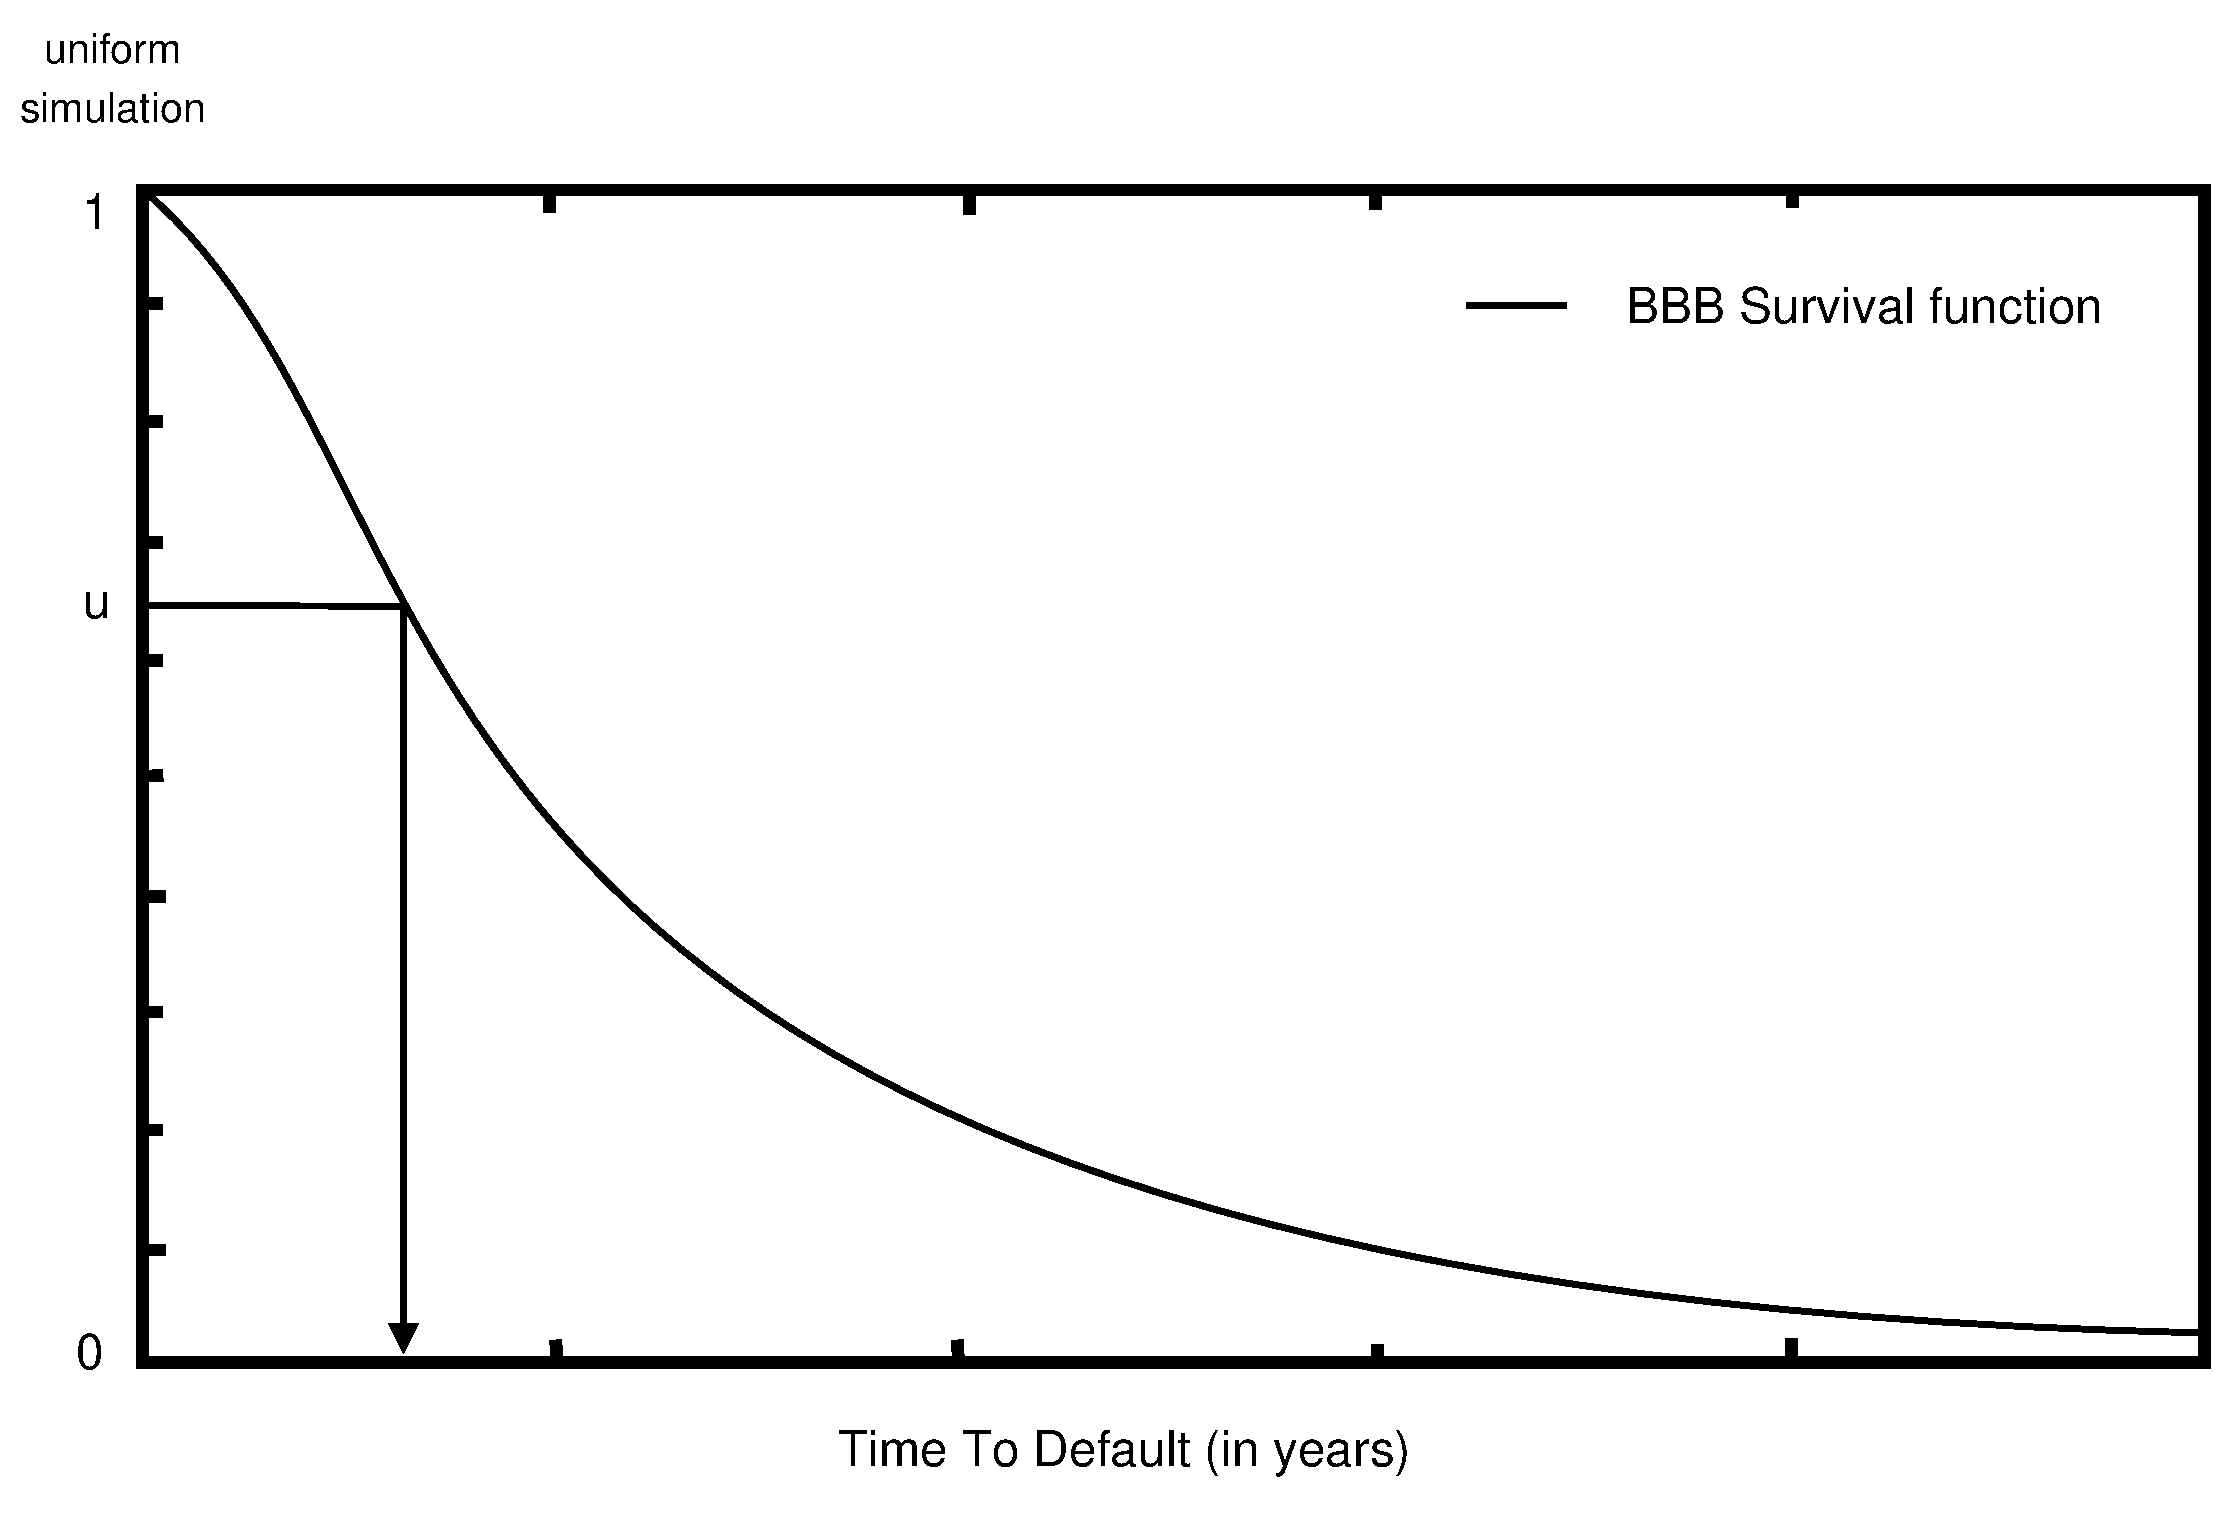
\includegraphics[width=10cm,angle=0]{./images/simttd.eps}
\caption{Simulaci\'on del tiempo hasta el fallido del rating $BBB$}
\label{simttd}
\end{center}
\end{figure}


\section{M\'etodo Rating-Path}
c\'opula -> matriz transici\'on -> valoraci\'on cartera

\begin{figure}[!hb]
\begin{center}
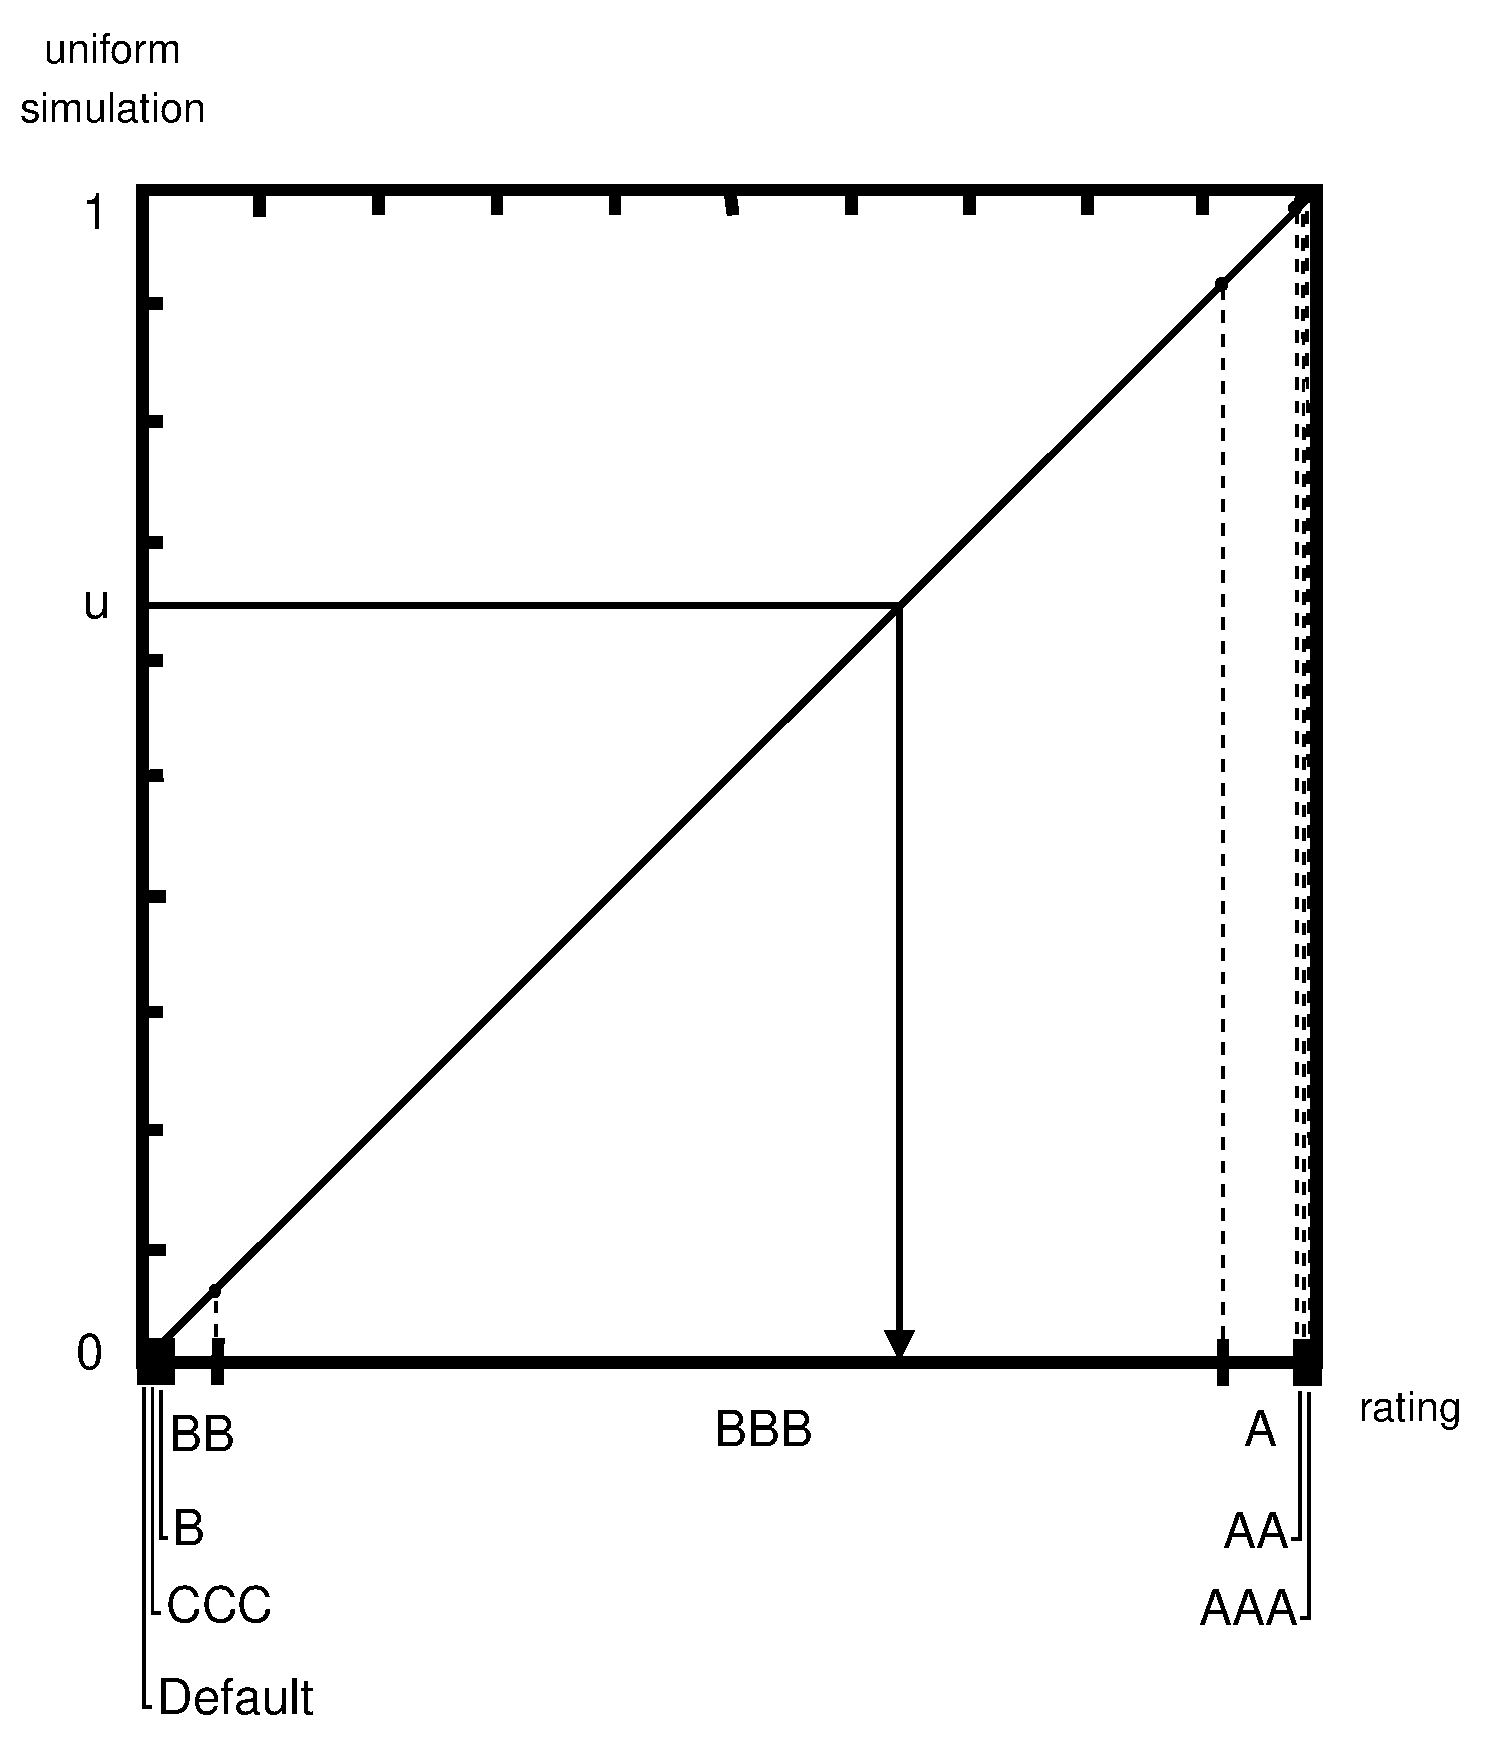
\includegraphics[width=7cm,angle=0]{./images/simrp.eps}
\caption{Simulaci\'on de la evoluci\'on del rating $BBB$ a $T$ tiempo}
\label{simrp}
\end{center}
\end{figure}


\subsection{Valoraci\'on de la cartera}
valoraci\'on activo -> valoraci\'on cliente -> valoraci\'on cartera

\subsection{Distribuci\'on del valor de la cartera}
calculo del valor esperado, calculo del VAR, etc.

